\documentclass[12 pt]{article}
\usepackage[left=2.66cm,top=3cm,right=2.66cm,bottom=3cm,bindingoffset=0.5cm]{geometry}

\usepackage{graphicx}
\usepackage{setspace}
\usepackage{enumitem}
\onehalfspacing

\begin{document}
\begin{titlepage}
\begin{Huge}
\begin{center}
\textsc{ RSA Algorithm \linebreak
and \linebreak
Public Key Cryptosystems}
\end{center}
\end{Huge}
\begin{center}
\begin{large}
\textsl{ Rohan Datta, Divya Raj}
\end{large}
\end{center}

\bigskip 
\begin{center}
\textbf{Abstract}
\end{center}
This text discusses the concept behind public key cryptosystems, while focusing on a very popular encryption method. It also presents an array of real world implementations of the algorithm.
Building upon ground-breaking research papers, it interprets the intriguing subject matter into an accessible form, and goes further to put forth their major applications and a few of their limitless possibilities.
\\
\\
\textit{Key words and phrases:} cryptosystems, discrete mathematics, encryption, decryption, prime numbers, digital signatures, public key cryptosystems, authentication, cyber security.
\end{titlepage}
\pagebreak
\begin{LARGE}	

\noindent \textbf{\textsc{Introduction to Public-Key Cryptography}}
\end{LARGE}

\noindent 
\\Public key cryptography, or asymmetrical cryptography, is any cryptographic system that uses pairs of keys: public keys which may be disseminated widely, and private keys which are known only to the owner. This accomplishes two functions: authentication, which is when the public key is used to verify that a holder of the paired private key sent the message, and encryption, whereby only the holder of the paired private key can decrypt the message encrypted with the public key.
\\\\The various methods that can and were used as alternatives to the public key systems are as follows:
\\\textbf{1. Symmetric}\\In a symmetric-key algorithm, both the sender and receiver share the key. The sender uses the key to hide the message. Then, the receiver will use the same key in the opposite way to reveal the message. For centuries, most cryptography has been symmetric. The problem with this system is that you have to make sure that the key is shared in a secure way, thus creating a chicken - egg problem.

\begin{figure}[h!]
  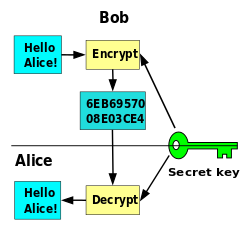
\includegraphics[width=55mm]{Symmetric_key_encryption.png}
  \centering
  \caption{Symmetric-key cryptography.}
  \label{fig:boat1}
\end{figure}
\noindent
\textbf{2. Decryption - Encryption in the middle}
\\In this system instead of having just two parties like above, one common third party(mostly a server) is added. So now, the sender and the server share a key(say K\textsubscript{a}), and the server and the receiver share a key(say K\textsubscript{b}). The sender's message is encrypted using K\textsubscript{a}, is decrypted at the server, then it is encrypted by K\textsubscript{b}, and sent to the receiver, where it finally gets decrypted and the message is delivered.

\noindent \textbf{{Introduction to public key cryptosystems}}
\end{LARGE}

\noindent 

\pagebreak
\begin{LARGE}
\noindent \textbf{{RSA Algorithm}}
\end{LARGE}\bigskip

\noindent RSA algorithm is an asymmetric cryptographic algorithm that is used extensively by computers nowadays. It was proposed by Ron Rivest, Adi Shamir and Leonard Adleman in their 1978 paper [reference], and hence, bears their name. It is one of the most popular implementations of public key cryptosystems.\bigskip

\noindent It is driven by the fact that finding the prime factors of a number is one of the most complex mathematical problems. Initially, the user creates and publishes the product of two large prime numbers, along with an auxiliary value. The auxiliary value takes up the role of the ``public key'' which is known to all. \emph{But, the prime factors must be kept secret.}\bigskip

1. Choose\ two\ different,\ large,\ random\  prime\  numbers\ \textbf{p} and \textbf{q}

2. Calculate \textbf{n} = \textbf{p}*\textbf{q}

3. \textbf{\boldmath $\phi(n)$ = (p - 1)*(q - 1)}

4. Choose an integer \textbf{e} such that:

\begin{itemize} \setlength\itemsep{1 em}
\setstretch{0.61803398875} \item  1 \textless \textbf{e} \textless \boldmath$\phi(n)$
\setstretch{0.61803398875} \item \textbf{e} is co-prime to \boldmath$\phi(n)$
\end{itemize}

5. Compute \textbf{d} such that \boldmath \textbf{d}*\textbf{e} = 1+\textbf{k}*\boldmath $\phi(n)$
\bigskip
\\
A popular choice for public exponents is \textbf{e} = $2$ \textsuperscript{$16$}+$1$

\end{document}


